\chapter{Evaluation}
\label{chapter:evaluation}

\section{Tests Objectives}

The test conducted were chosen because they have direct contribution with this thesis goals.

Our system leverages user detection to improve occupant comfort and reduce wasted energy and because of that we require the user detection to have medium/low accuracy in building detection time and high accuracy in room detection.



%In order to evaluate the developed system, several tests were performed. Section 5.1 starts by describing
%the test scenario. Next, in Section 5.2 the detailed description of each test is presented. Finally,
%Section 5.3 presents the results of the tests.

\section{Tests Scenarios}



All the tests were conducted in real scenarios inside a office of the IST - Taguspark campus. They
were executed using the hardware described in Section~\ref{hardware_arch_imp} and one Moto G3 phone running the user app.


\subsection{User detection - Room}

3 tipos de teste:
tempo que demora a detectar dentro do gabinete e se o tempo é aceitavel para ligar luzes ou ar condicionado;
fazer mediçoes do range do beacon para saber se no gabinete ao lado ele acusa erradamente que estou no gabinete.




In order to test the reaction time of user detection in the office, a series of measurements were performed. The test consists in observing the time the user app takes to detect the Estimote beacon present inside the office. The user will start walking from just outside the beacon range and walk normally to the office door.

The measurements will be performed with the beacon device near the door in order to increase signal range outside the office. The device used will be a Moto G3 Android phone with BT support up to version 4.0 .
For testing purposes the user app is set to vibrate when it near the beacon in order for us to know if it found the beacon, a chronometer will be used to determine the reaction time. The test will result in at least a set of 25 measurements in order to determine a meaningful average of the reaction time of the system.


\subsection{User detection - Building}

se houver tempo ter X pessoas com a app instalada para medir ao fim de 3 dias se os utilizadores estavam no edificio às horas registadas.
Ou medir o tempo que demora ate detectar que que esta no edificio.


In order to test the reaction time of user detection in the building, a series of measurements were performed. The test consists in observing the time the user app takes to detect phone is inside the building. The user will start walking from the front door to the building and normally to the office door.

The device used will be a Moto G3 Android phone with WiFi support.
For testing purposes the user app is set to vibrate when it is inside the building, a chronometer will be used to determine the reaction time. The test will result in at least a set of 25 measurements in order to determine a meaningful average of the reaction time of the system.



\subsection{Motion detection}

(testar com pessoas diferentes)

(mostrar as imagens com as diferenças)

To test the motion detection a series of measurements were performed to test the algorithm. The test consists in a person walking in front of the Hub camera at different speeds from the door to a desk. This test will show if our system is able to detect motion when people enter the office and if it can be tricked and produce wrong negatives.




\subsection{Temperature and Luminosity}

medir a luminosidade e ligar uma luz e mostrar o grafico da alteração.


\subsection{Hub server load}

(stress test)

To test our system web-server a series of measures were performed. This test consists in making several concurrent \ac{HTTP} requests.

 concurring requests to our \ac{API} 


\subsection{Automation}
testes com utilizadores a criar receitas



Nesta secção devem descrever o cenário de teste, incluindo, por exemplo, a
definição da rede, o modelo de tráfego, as características de cada elemento....
A descrição deve ser feita, de forma a que os testes possam ser reprodutíveis.
Se os testes forem feitos em ambiente real devem ser descritas as características
dos equipamentos, memória, CPU, disco, SO, etc....

Devem também descrever as características das experiências, do ponto de vista
estatístico. Número de testes realizados, grandezas que vão ser medidas, formas de
medição dos valores, etc...

Sempre que possível, ilustrem o cenário de testes com figuras e com tabelas, que
descrevam sucintamente o modelo.

\section{Test Results}


\subsection{User detection - Room}

A set of measurements were taken in order to determine the response time the application takes to identify the user's phone is inside the room. Two types of measurements were taken.

In the first the user is inside the room with \ac{BT} turned off, then it was turned on and timer started, column 1 of Table~\ref{eval:room} shows the measurements obtained. 

In the second set of measurements the user starts walking outside the office and opens a unlocked door to the room.


\begin{table}[]
\centering
\begin{tabular}{|l|l|}
\hline
\begin{tabular}[c]{@{}l@{}}Time (seconds) to detect user \\ presence in room, when user \\ is already inside\end{tabular} &  \\ \hline
2.13 &  \\ \hline
2.23 &  \\ \hline
2.02 &  \\ \hline
23.55 &  \\ \hline
6.65 &  \\ \hline
11.5 &  \\ \hline
7.16 &  \\ \hline
2.36 &  \\ \hline
2.18 &  \\ \hline
2.48 &  \\ \hline
12.4 &  \\ \hline
2.15 &  \\ \hline
6.73 &  \\ \hline
2.18 &  \\ \hline
11.93 &  \\ \hline
2.22 &  \\ \hline
2.12 &  \\ \hline
16.62 &  \\ \hline
2.08 &  \\ \hline
2.23 &  \\ \hline
\end{tabular}
\caption{Room detection - evaluation}
\label{eval:room}
\end{table}

\subsection{Motion detection}

To test our motion detection algorithm and system, we conducted tests with three different people with different heights. Each person entered the room at different speeds, the obtained results are shown in Table~\ref{eval:motion}.

Our system was able to correctly identify a person walking inside the room every time, Figure~\ref{eval:motion_fig} shows the different pixels in the camera frames identified by our algorithm. Regarding false positives, they don't seem to be a problem since our system allow the creation of a no monitoring area in the camera frame to use in cases of rooms with window view.


\begin{table}[]
\centering
\begin{tabular}{|l|l|l|l|}
\hline
 & \begin{tabular}[c]{@{}l@{}}Person 1\\ detection\end{tabular} & \begin{tabular}[c]{@{}l@{}}Person 2\\ detection\end{tabular} & \begin{tabular}[c]{@{}l@{}}Person 3\\ detection\end{tabular} \\ \hline
Slow walk & 20/20 & 20/20 & 20/20 \\ \hline
Normal walk & 20/20 & 20/20 & 20/20 \\ \hline
Run & 20/20 & 20/20 & 20/20 \\ \hline
\end{tabular}
\caption{Motion detection tests for three people with different heights, 20 measurements each.}
\label{eval:motion}
\end{table}


\begin{figure}[h]
\centering
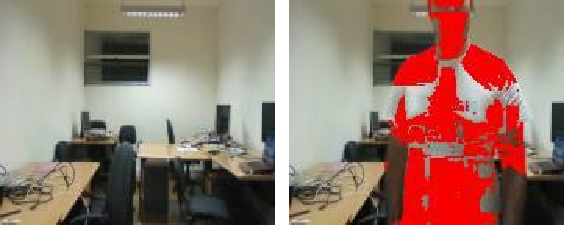
\includegraphics[width=0.4\textwidth]{Figures/eval_motion}
\caption{Motion detection - Frame before and after, motion detected }
\label{eval:motion_fig}
\end{figure}


